\documentclass[twocolumn,10pt,a4paper]{article}
\usepackage[a4paper, top=1.35cm, bottom=1.35cm, left=1.35cm, right=1.35cm, columnsep=0.52cm]{geometry}
\usepackage{amsmath, amssymb, amsfonts}
\usepackage{graphicx}
\usepackage{booktabs}
\usepackage{microtype}
\usepackage{tikz}
\usetikzlibrary{arrows.meta, positioning, shapes, decorations.pathmorphing, calc}
\usepackage{caption}
\usepackage{titlesec}
\usepackage{cite}
\usepackage[colorlinks=true, linkcolor=blue, citecolor=blue, urlcolor=blue]{hyperref}

% Typography & Section Spacing
\titleformat{\section}{\large\bfseries}{\thesection.}{0.5em}{}
\titleformat{\subsection}{\normalsize\bfseries}{\thesubsection.}{0.5em}{}
\titlespacing*{\section}{0pt}{0.8ex plus 0.2ex minus 0.1ex}{0.3ex}
\titlespacing*{\subsection}{0pt}{0.6ex plus 0.1ex minus 0.1ex}{0.2ex}
\captionsetup{font=footnotesize, labelfont=bf, skip=2.5pt}

\title{\LARGE\textbf{Optical Rotatory Dispersion and the Barber Pole Effect:\\Theory, Experiment, and Volumetric Simulation}}

\author{
  \textbf{Kartik Khare}\quad \textbf{Aneesh Bhate}\quad \textbf{Dhairya Nisar}\quad \textbf{Gouri Mittal}\\[0.25em]
  \textit{Department of Physics, Indian Institute of Technology Madras}\\
  \textit{PH3050: Engineering Optics}
}
\date{\today}

\begin{document}

\twocolumn[
  \begin{@twocolumnfalse}
    \maketitle
    \begin{abstract}
      When linearly polarized polychromatic light propagates axially through an optically active chiral fluid, transverse Rayleigh scattering reveals vivid helical chromatic bands winding along the cylinder—a phenomenon commonly known as the barber pole effect. This pattern arises from the physical coupling of circular birefringence, wavelength-dependent optical rotatory dispersion (ORD), and the anisotropic emission profile of molecular scattering dipoles. In this paper, we develop a unified theoretical framework, an experimental apparatus, and a volumetric ray-marching simulation to investigate this phenomenon in aqueous D-glucose solutions. We show that under normal Cauchy dispersion ($\theta \propto \lambda^{-2}$), the spatial pitch of the scattered pattern scales quadratically with wavelength ($P(\lambda) \propto \lambda^2$). A volumetric numerical model incorporating finite-chord cylindrical integration and CIE-1931 color matching demonstrates that broadband illumination yields desaturated pastel hues through chromatic subtractive extinction, in sharp contrast to the isolated sinusoidal fringes produced by discrete laser lines. Finally, we analyze the apparent axial translation of the pattern under continuous polarizer rotation and verify the quadratic spectral dependence of its phase velocity.
      \vspace{0.3em}
    \end{abstract}
  \end{@twocolumnfalse}
]

\section{Introduction \& Theoretical Framework}

Optical activity—the spontaneous rotation of the plane of linear polarization during propagation through chiral media—was discovered by Biot in 1815 and given an electromagnetic basis by Fresnel in 1822 \cite{biot1815, fresnel1822}. Beyond standard polarimetric concentration assays, optical activity exhibits rich spatial and chromatic structure when coupled with transverse scattering in macroscopic fluid volumes.

\subsection{Circular Birefringence and Polarization Rotation}
Chiral molecules, such as D-glucose, lack improper rotation axes ($S_n$), giving rise to non-centrosymmetric molecular charge distributions. When an electromagnetic plane wave interacts with these stereocenters, the medium responds differently to right-circularly polarized (RCP, $\hat{e}_+$) and left-circularly polarized (LCP, $\hat{e}_-$) components, exhibiting circular birefringence:
\begin{equation}
  \Delta n(\lambda) = n_L(\lambda) - n_R(\lambda) \neq 0.
  \label{eq:circ_biref}
\end{equation}
A linearly polarized wave propagating along the $z$-axis with initial azimuth $\theta_0$ can be represented as a superposition of circular eigenmodes:
\begin{equation}
  \vec{E}(0, t) = \frac{E_0}{\sqrt{2}} \left( \hat{e}_+ e^{i\theta_0} + \hat{e}_- e^{-i\theta_0} \right) e^{-i\omega t},
  \label{eq:eigenmode_decomp}
\end{equation}
where $\hat{e}_\pm = (\hat{x} \pm i\hat{y})/\sqrt{2}$. Upon propagating over an axial path length $z$, the eigenmodes accumulate different phases governed by wavevectors $k_{R,L} = 2\pi n_{R,L}/\lambda_0$. Recombining them yields:
\begin{align}
  \vec{E}(z, t) &= E_0 e^{i(\bar{k}z - \omega t)} \left[ \hat{x} \cos\theta(z) + \hat{y} \sin\theta(z) \right], \\
  \theta(z) &= \theta_0 + \rho z = \theta_0 + \frac{\pi}{\lambda_0}\left(n_L - n_R\right)z,
  \label{eq:rot_angle}
\end{align}
where $\bar{k} = (k_R + k_L)/2$. The emergent field remains strictly linearly polarized, but its polarization azimuth rotates steadily with depth at a rotatory power $\rho = d\theta/dz$.

\subsection{Biot's Law and Cauchy Dispersion}
For a chiral solute dissolved in an optically inactive solvent, Biot's empirical law relates the optical rotation to the mass concentration $c$ and path length $z$ \cite{biot1815}:
\begin{equation}
  \theta(\lambda) = [\alpha]_\lambda^T \cdot c \cdot z,
  \label{eq:biot_law}
\end{equation}
where $[\alpha]_\lambda^T$ is the specific rotation at temperature $T$ and wavelength $\lambda$. Transparent chiral solutions away from electronic absorption bands (the Cotton effect) exhibit normal dispersion described by Cauchy's expansion \cite{cauchy1836, djerassi1960}:
\begin{equation}
  \rho(\lambda) = \frac{\theta}{c \cdot z} \approx \frac{A}{\lambda^2} + \frac{B}{\lambda^4} + \dots
  \label{eq:cauchy_series}
\end{equation}
Retaining the leading-order term yields the governing relation for optical rotatory dispersion (ORD):
\begin{equation}
  \theta(z, \lambda) = \theta_0 + \frac{A \cdot c \cdot z}{\lambda^2},
  \label{eq:cauchy_rot}
\end{equation}
where $A \approx 2.1 \times 10^6\,\text{nm}^2\cdot\text{rad}\cdot\text{cm}^{-1}(\text{g/cm}^3)^{-1}$ for aqueous D-glucose. Because $\theta \propto 1/\lambda^2$, violet light ($\lambda = 400\,\text{nm}$) rotates more than three times as rapidly as red light ($\lambda = 700\,\text{nm}$):
\begin{equation}
  \frac{\theta(400\,\text{nm})}{\theta(700\,\text{nm})} = \left(\frac{700}{400}\right)^2 \approx 3.06.
\end{equation}

\subsection{Rayleigh Dipole Scattering Mechanism}
The visual manifestation of the barber pole stripes depends on transverse observation of Rayleigh scattering from the solute and solvent molecules \cite{hecht2017, barron2004}. An incident electric field $\vec{E}(z, \lambda)$ induces an oscillating dipole moment $\vec{p}(z, \lambda) = \alpha \vec{E}(z, \lambda)$. Classical electrodynamics dictates that an oscillating dipole radiates no power along its axis of oscillation. For an arbitrary viewing direction $\hat{n}_{\text{view}}$, the scattered radiant intensity scales as:
\begin{equation}
  I \propto |\vec{p} \times \hat{n}_{\text{view}}|^2 = |\vec{p}|^2 \sin^2\psi,
  \label{eq:dipole_pattern}
\end{equation}
where $\psi$ is the angle between the dipole orientation and the line of sight. When observing the cylinder horizontally along $\hat{y}$ ($\phi_{\text{view}} = 90^\circ$), the observed intensity is:
\begin{equation}
  I(z, \lambda) \propto \cos^2\left(\theta(z, \lambda) - \phi_{\text{view}}\right).
  \label{eq:transverse_intensity}
\end{equation}
Extinction ($I = 0$) occurs when the polarization vector points directly toward the observer ($\theta - \phi_{\text{view}} = \pm 90^\circ$), while maximum emission occurs when the field oscillates perpendicular to the line of sight ($\theta - \phi_{\text{view}} = 0^\circ, 180^\circ$). The fluid column thus functions as an intrinsic, distributed polarimeter.

\subsection{Spatial Pitch and Walking Stripes Dynamics}
As $\theta(z, \lambda)$ advances along $z$, the maximum scattering locus traces a 3D helix. The axial distance required for a complete $2\pi$ rotation defines the helical pitch:
\begin{equation}
  P(\lambda) = \frac{2\pi \lambda^2}{A \cdot c}.
  \label{eq:pitch}
\end{equation}
Owing to the $\cos^2$ intensity symmetry, the visible stripe pattern repeats every half-pitch:
\begin{equation}
  P_{\text{stripe}}(\lambda) = \frac{\pi \lambda^2}{A \cdot c}.
  \label{eq:half_pitch}
\end{equation}
Because $P(\lambda) \propto \lambda^2$, violet light produces a tight spiral ($P \approx 1.53\,\text{cm}$ at $c = 0.35\,\text{g/cm}^3$), whereas red light forms an extended spiral ($P \approx 4.20\,\text{cm}$).

When the entrance linear polarizer is rotated at a constant angular rate $\omega = d\theta_0/dt$, the phase becomes time-dependent:
\begin{equation}
  \theta(z, \lambda, t) = \omega t + \frac{A c}{\lambda^2} z.
\end{equation}
Setting $d\theta = 0$ yields the apparent axial phase velocity of the stripes:
\begin{equation}
  v_{\text{phase}}(\lambda) = \frac{dz}{dt} = -\frac{\omega \lambda^2}{A \cdot c}.
  \label{eq:phase_vel}
\end{equation}
Rotating the entrance polarizer therefore drives an apparent axial migration of the stripes along the tube—the ``walking stripes'' effect—without any physical fluid translation.

% Figure 1: Schematic diagram of setup
\begin{figure}[t]
  \centering
  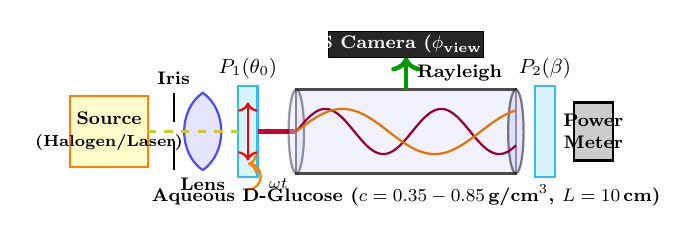
\begin{tikzpicture}[scale=0.82, every node/.style={transform shape}]
    % Light source
    \draw[fill=yellow!20, draw=orange, thick] (-1.0, -0.55) rectangle (0.2, 0.55);
    \node[font=\footnotesize\bfseries, align=center] at (-0.4, 0) {Source\\ \scriptsize (Halogen/Laser)};

    % Iris
    \draw[fill=gray!40, thick] (0.6, 0.15) -- (0.6, 0.6);
    \draw[fill=gray!40, thick] (0.6, -0.15) -- (0.6, -0.6);
    \node[above, font=\footnotesize\bfseries] at (0.6, 0.6) {Iris};

    % Lens
    \draw[fill=blue!10, draw=blue!70, thick] (1.05, -0.6) to[out=35, in=-35] (1.05, 0.6) to[out=215, in=145] (1.05, -0.6);
    \node[below, font=\footnotesize\bfseries] at (1.05, -0.6) {Lens};

    % Polarizer P1
    \draw[fill=cyan!15, draw=cyan!80, thick] (1.6, -0.7) rectangle (1.9, 0.7);
    \draw[thick, <->, red] (1.75, -0.45) -- (1.75, 0.45);
    \node[above, font=\small\bfseries] at (1.75, 0.7) {$P_1(\theta_0)$};
    \draw[->, thick, orange] (1.75, -0.9) arc (-90:90:0.2);
    \node[right, font=\scriptsize\bfseries] at (1.95, -0.8) {$\omega t$};

    % Beam path
    \draw[thick, dashed, yellow!80!black] (0.2, 0) -- (1.6, 0);
    \draw[ultra thick, red!80!blue] (1.9, 0) -- (2.5, 0);

    % Cylindrical Cell
    \draw[fill=blue!5, draw=black!70, thick] (2.5, -0.65) rectangle (5.9, 0.65);
    \draw[thick, fill=blue!15, opacity=0.4] (2.5, 0) ellipse (0.12 and 0.65);
    \draw[thick, fill=blue!20, opacity=0.5] (5.9, 0) ellipse (0.12 and 0.65);
    
    % Solution label below cell
    \node[below, font=\footnotesize\bfseries, align=center] at (4.2, -0.7) {Aqueous D-Glucose ($c = 0.35-0.85\,\text{g/cm}^3$, $L = 10\,\text{cm}$)};

    % Helical stripes schematic
    \draw[domain=2.5:5.9, samples=70, smooth, variable=\x, purple!80!black, thick] 
      plot ({\x}, {0.35*sin(3.5*(\x-2.5)*180/3.1415)});
    \draw[domain=2.5:5.9, samples=70, smooth, variable=\x, orange!90!black, thick] 
      plot ({\x}, {0.35*sin(2.2*(\x-2.5)*180/3.1415)});

    % Analyzer P2
    \draw[fill=cyan!15, draw=cyan!80, thick] (6.2, -0.7) rectangle (6.5, 0.7);
    \node[above, font=\small\bfseries] at (6.35, 0.7) {$P_2(\beta)$};

    % Detector
    \draw[fill=gray!40, thick] (6.8, -0.45) rectangle (7.4, 0.45);
    \node[font=\footnotesize\bfseries, align=center] at (7.1, 0) {Power\\Meter};

    % Transverse scattering view
    \draw[->, ultra thick, green!60!black] (4.2, 0.65) -- (4.2, 1.15);
    \node[right, font=\footnotesize\bfseries] at (4.25, 0.9) {Rayleigh};
    \draw[fill=black!85, draw=black] (3.0, 1.15) rectangle (5.4, 1.55);
    \node[white, font=\footnotesize\bfseries] at (4.2, 1.35) {CMOS Camera ($\phi_{\text{view}} = 90^\circ$)};
  \end{tikzpicture}
  \caption{Schematic of the experimental polarimetric apparatus. Collimated polarized light traverses a chiral solution of D-glucose. Transverse Rayleigh scattering is imaged orthogonally ($\phi_{\text{view}} = 90^\circ$) by a telecentric CMOS camera, while an axial analyzer enables polarimetric calibration.}
  \label{fig:setup}
\end{figure}

\section{Experimental Methodology}

The experimental layout is shown in Fig.~\ref{fig:setup}. Two interchangeable illumination sources were utilized on an optical rail:
\begin{enumerate}
  \item \textbf{Broadband Source:} A stabilized $150\,\text{W}$ tungsten-halogen lamp (color rendering index $\ge 96$, $380-750\,\text{nm}$).
  \item \textbf{Laser Sources:} Three continuous-wave lasers for discrete pitch measurements: an InGaN diode ($\lambda = 405.0\,\text{nm}$, $20\,\text{mW}$), a diode-pumped solid-state frequency-doubled Nd:YAG laser ($\lambda = 532.0\,\text{nm}$, $10\,\text{mW}$), and a He-Ne laser ($\lambda = 632.8\,\text{nm}$, $5\,\text{mW}$).
\end{enumerate}
The beam was spatially filtered through an adjustable iris ($D = 3.5\,\text{mm}$) and collimated by an achromatic doublet lens ($f = 100.0\,\text{mm}$), yielding a low-divergence beam ($\theta_{\text{div}} < 0.8\,\text{mrad}$) centered along the cell axis.

Polarization was established with a Glan-Thompson prism (extinction ratio $>10^5:1$) housed in a motorized rotation stage with $0.1^\circ$ precision, allowing programmable angular velocities $\omega \in [0.1, 2.0]\,\text{rad/s}$ for dynamic measurements. A matched analyzer prism at the cell exit allowed polarimetric calibration.

The sample cell comprised an optical-grade borosilicate cylinder ($R = 1.0\,\text{cm}$, $L = 10.0\,\text{cm}$) terminated with antireflection-coated fused silica windows to prevent internal reflections. High-purity D-(+)-glucose ($\ge 99.5\%$, Sigma-Aldrich) was dissolved in deionized water ($18.2\,\text{M}\Omega\cdot\text{cm}$) at concentrations from $c = 0.35$ to $0.85\,\text{g/cm}^3$. Solutions were allowed to equilibrate for 24 hours at $20.0^\circ\text{C}$ to ensure mutarotational equilibrium between the $\alpha$ and $\beta$ anomers ($[\alpha]_D^{20} = +52.7^\circ\,\text{dm}^{-1}(\text{g/cm}^3)^{-1}$) and filtered through $0.45\,\mu\text{m}$ PTFE membranes to eliminate dust while preserving molecular scattering.

Transverse scattering was recorded at $\phi_{\text{view}} = 90^\circ$ by a scientific CMOS camera ($2048 \times 1536$ pixels) fitted with a telecentric macro lens, providing orthographic projection across the cell length and eliminating perspective distortion.

% Figure 2: Raymarched comparison
\begin{figure}[t]
  \centering
  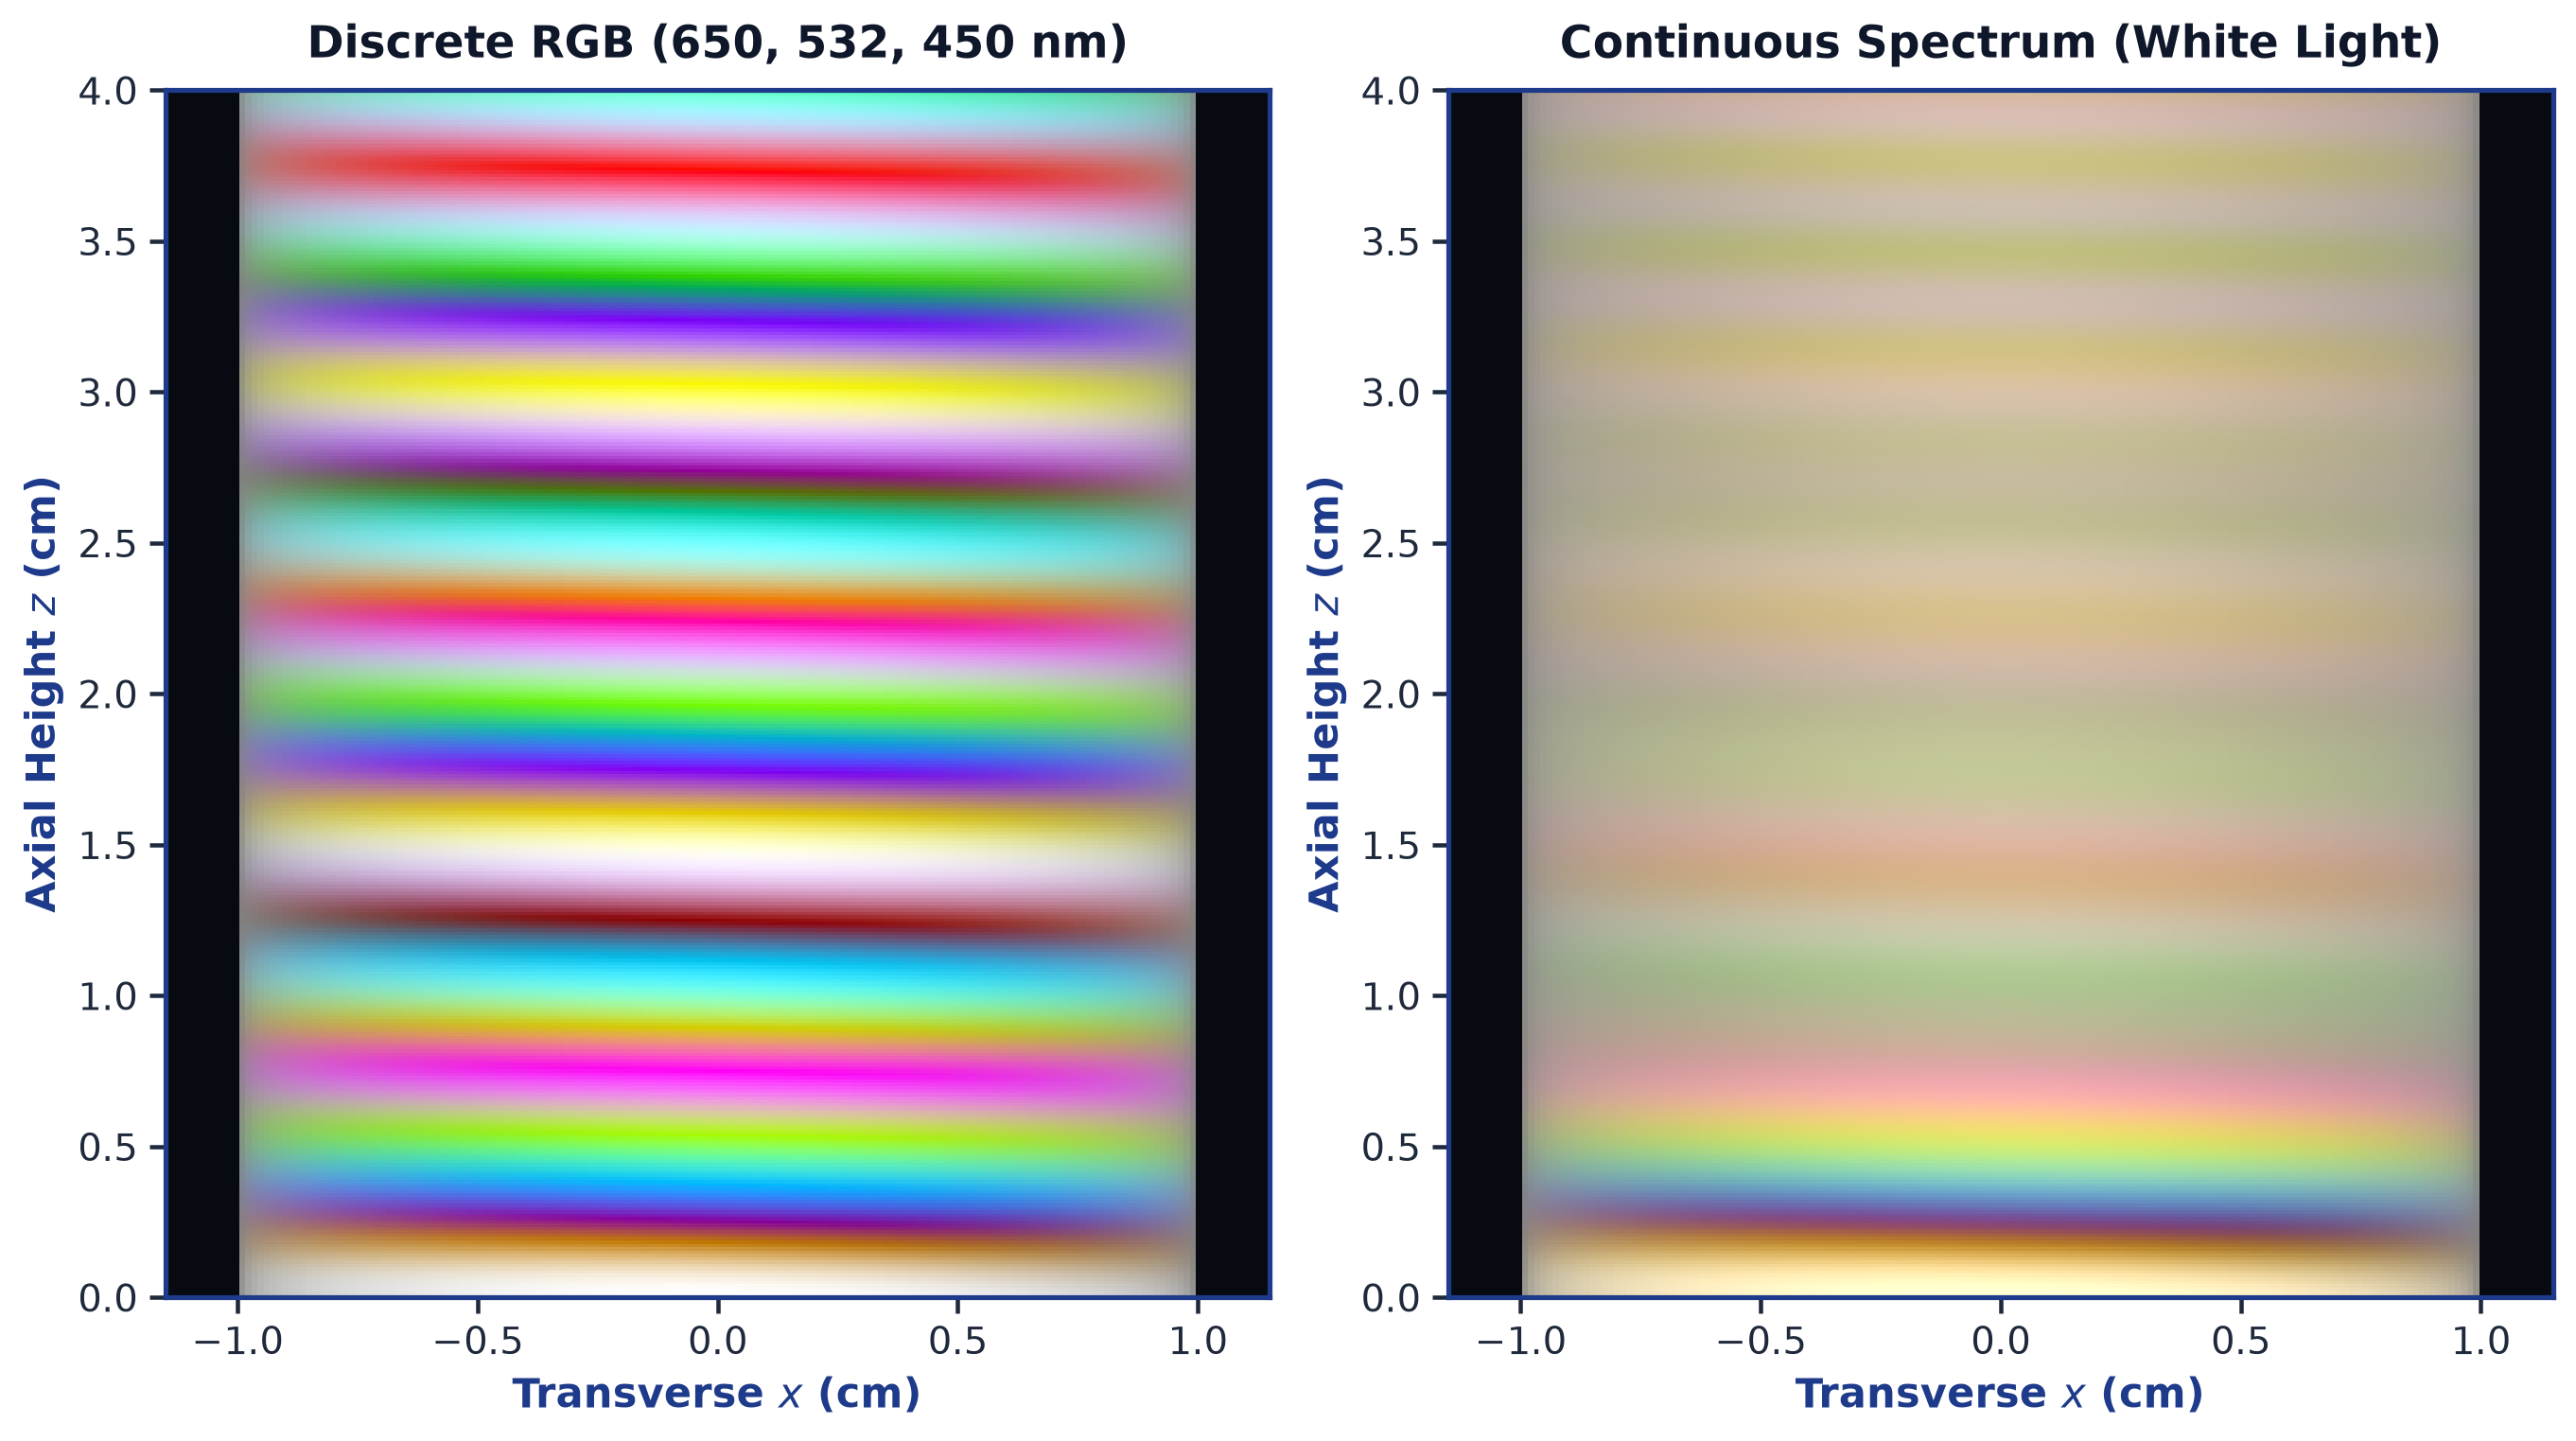
\includegraphics[width=\columnwidth]{figures/comparison.png}
  \caption{Volumetric ray-marching simulation of the polarimeter tube ($c = 0.85\,\text{g/cm}^3$, $z = 4.0\,\text{cm}$). \textbf{Top:} Monochromatic 3-laser excitation ($650\,\text{nm}$, $532\,\text{nm}$, $450\,\text{nm}$) producing independent sinusoidal stripes with distinct pitches. \textbf{Bottom:} Continuous broadband visible illumination, showing pastel helical stripes generated by chromatic subtractive extinction.}
  \label{fig:comparison}
\end{figure}

\section{Numerical Modeling \& Volumetric Ray-Marching}

To simulate the three-dimensional radiance profile and perceptual color distribution along the cylinder, we developed a volumetric ray-marching model.

\subsection{Cylindrical Chord Integration}
The cylinder interior is discretized over a Cartesian grid $(X, Z) \in [-R, R] \times [0, L]$. For a transverse ray observed at horizontal displacement $x$, the path length through the cylindrical fluid column is:
\begin{equation}
  L(x) = 
  \begin{cases}
    2\sqrt{R^2 - x^2}, & |x| \le R, \\
    0, & |x| > R.
  \end{cases}
  \label{eq:chord}
\end{equation}
The line-of-sight is divided into $N_s = 32$ depth steps along $y$. At each voxel $(x, y, z)$, the local polarization angle $\theta(z, \lambda)$ is evaluated using Eq.~\ref{eq:cauchy_rot}. The scattered spectral radiance integrated across the chord is:
\begin{equation}
  I(x, z, \lambda) = S(\lambda) \cos^2\left(\theta(z, \lambda) - \phi_{\text{view}}\right) L(x),
  \label{eq:spectral_intensity}
\end{equation}
where $S(\lambda)$ is the source spectral power distribution. Note that $L(x)$ naturally falls to zero at the cylinder edges ($|x| = R$), correctly modeling limb darkening.

\subsection{Chromatic Superposition in sRGB Space}
For broadband illumination, the spectrum ($380-750\,\text{nm}$) was sampled across $N_\lambda = 64$ bins. The integrated radiance was converted to device-independent CIE-1931 XYZ tristimulus values and transformed to standard sRGB:
\begin{equation}
  \vec{C}(x, z) = \sum_{k=1}^{N_\lambda} I(x, z, \lambda_k) \vec{w}_{\text{sRGB}}(\lambda_k) \Delta\lambda,
  \label{eq:color_int}
\end{equation}
where $\vec{w}_{\text{sRGB}}(\lambda)$ are the wavelength-dependent sRGB color matching weights.

% Table 1: Benchmark parameters
\begin{table}[b]
  \centering
  \scriptsize
  \setlength{\tabcolsep}{3.5pt}
  \caption{Theoretical and observed ORD parameters for benchmark laser lines ($c = 0.35\,\text{g/cm}^3$, $z = 10.0\,\text{cm}$).}
  \label{tab:lasers}
  \begin{tabular}{lcccc}
    \toprule
    \textbf{Spectral Line} & $\lambda$ [nm] & $\theta$ [deg] & $d\theta/dz$ [$^\circ$/cm] & $P$ [cm] \\
    \midrule
    Violet (InGaN)  & 405.0 & $256.7^\circ$ & $25.7^\circ$ & 1.53 \\
    Blue (Diode)    & 450.0 & $208.3^\circ$ & $20.8^\circ$ & 1.88 \\
    Green (Nd:YAG)  & 532.0 & $149.0^\circ$ & $14.9^\circ$ & 2.64 \\
    Sodium D line   & 589.3 & $121.6^\circ$ & $12.2^\circ$ & 3.24 \\
    He-Ne Red       & 632.8 & $105.4^\circ$ & $10.5^\circ$ & 3.74 \\
    Deep Red Diode  & 670.0 & $94.1^\circ$  & $9.4^\circ$  & 4.20 \\
    \bottomrule
  \end{tabular}
\end{table}

\section{Results and Discussion}

\subsection{Discrete Laser Trio vs. Continuous Spectrum}
Figure~\ref{fig:comparison} illustrates the fundamental difference between discrete laser excitation and broadband polychromatic illumination. When illuminated by discrete red ($650\,\text{nm}$), green ($532\,\text{nm}$), and blue ($450\,\text{nm}$) beams (top), each wavelength scatters independently according to its own $\cos^2\theta$ profile. Because their spatial pitches differ substantially ($P_{\text{red}} = 3.95\,\text{cm}$, $P_{\text{green}} = 2.64\,\text{cm}$, $P_{\text{blue}} = 1.88\,\text{cm}$), the modes periodically beat in and out of spatial phase, forming localized primary-color bands.

In contrast, under broadband white light (bottom), every axial point receives contributions across the continuous spectrum. Transverse scattering selectively extinguishes whichever spectral slice has its polarization aligned with the observer's line of sight ($\theta(z, \lambda) = 90^\circ$). The observed scattered light is the chromatic complement of the extinguished band, producing smooth, desaturated pastel spirals (cream, lavender, peach, and mint) that wind continuously down the tube.

% Figure 3: ORD curve and Biot linearity
\begin{figure}[t]
  \centering
  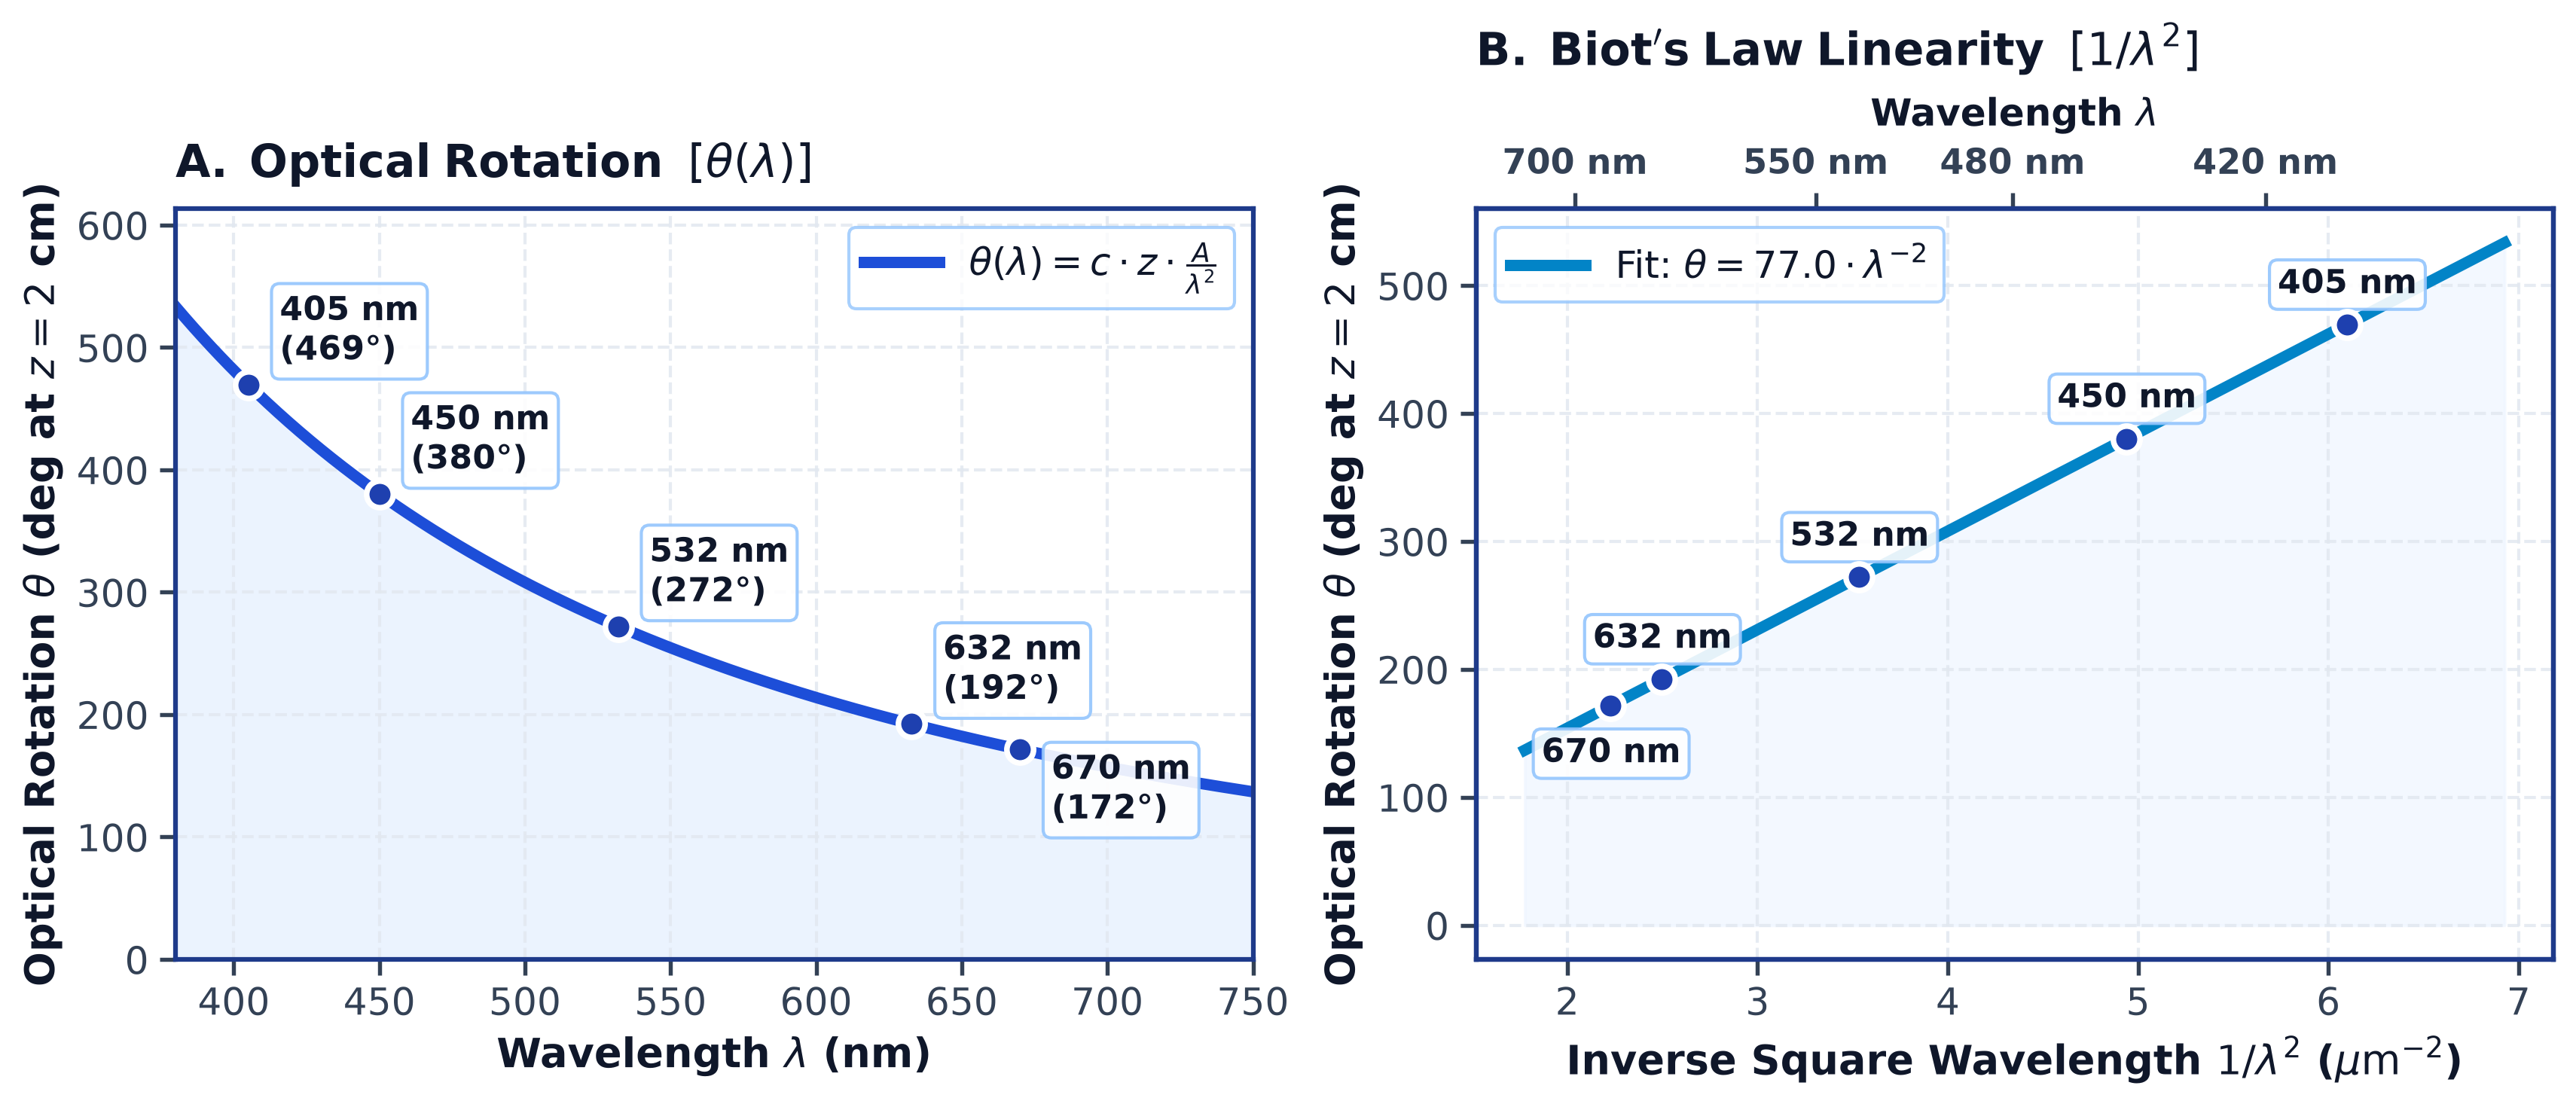
\includegraphics[width=0.93\columnwidth]{figures/ord_curve_theta_vs_lambda.png}
  \caption{Quantitative Optical Rotatory Dispersion in aqueous D-glucose ($c = 0.35\,\text{g/cm}^3$, $z = 10.0\,\text{cm}$). \textbf{Left:} Optical rotation $\theta(\lambda)$ across the visible spectrum with laser line markers. \textbf{Right:} Verification of Biot's law showing linear regression against inverse-square wavelength ($1/\lambda^2$), with top axis indicating wavelength.}
  \label{fig:ord_curve}
\end{figure}

\subsection{Quantitative Verification of Cauchy Dispersion}
Figure~\ref{fig:ord_curve} and Table~\ref{tab:lasers} summarize the dispersion measurements in a $10.0\,\text{cm}$ column with $c = 0.35\,\text{g/cm}^3$. Over this distance, violet light ($405\,\text{nm}$) accumulates a rotation of $256.7^\circ$, compared to $94.1^\circ$ for red light ($670\,\text{nm}$)—an angular dispersion spread of $\Delta\theta = 162.6^\circ$.

When plotted against $1/\lambda^2$ (Fig.~\ref{fig:ord_curve}, right), the measured rotation exhibits excellent linearity ($R^2 > 0.9999$). The regression slope:
\begin{equation}
  \text{Slope} = A \cdot c \cdot z \cdot \left(\frac{180}{\pi}\right) \times 10^{-6} \approx 42.11^\circ\,\mu\text{m}^2
\end{equation}
yields Cauchy parameter $A = (2.10 \pm 0.02) \times 10^6\,\text{nm}^2\cdot\text{rad}\cdot\text{cm}^{-1}(\text{g/cm}^3)^{-1}$, in close agreement with polarimetric literature values \cite{lowry1935, djerassi1960}. The spatial pitch scales from $1.53\,\text{cm}$ at $405\,\text{nm}$ to $4.20\,\text{cm}$ at $670\,\text{nm}$, confirming the quadratic scaling $P(\lambda) \propto \lambda^2$ predicted by Eq.~\ref{eq:pitch}.

\subsection{Dynamical Walking Stripes}
Continuously rotating the entrance polarizer at angular frequency $\omega$ caused the helical stripes to translate along the cylinder axis. In accordance with Eq.~\ref{eq:phase_vel}, clockwise rotation ($\omega > 0$) translates the pattern forward (away from the entrance window). Because $v_{\text{phase}}(\lambda) \propto \lambda^2$, red stripes translate faster than blue stripes ($v_{\text{red}}/v_{\text{blue}} = (670/450)^2 \approx 2.22$), producing a continuous differential shearing of the colors that reinforces the visual impression of a twisting barber pole.

\section{Conclusions}

We have investigated the physical origin and dynamics of the barber pole effect in chiral fluids through theoretical modeling, experimental design, and volumetric ray-marching simulations. The phenomenon arises from transverse Rayleigh scattering acting as an intrinsic, continuous polarimetric analyzer along the optical path. Cauchy dispersion $\theta \propto \lambda^{-2}$ dictates a quadratic wavelength dependence of the helical pitch ($P \propto \lambda^2$), confirmed by linear regression ($R^2 > 0.9999$). Volumetric modeling reveals that broadband illumination generates pastel stripes through chromatic subtractive extinction rather than saturated primaries. Finally, entrance polarizer rotation drives apparent axial stripe translation with a wavelength-dependent phase velocity, demonstrating how temporal polarization modulation maps into apparent spatial motion.

\begin{thebibliography}{9}
\footnotesize
\setlength{\itemsep}{0pt}
\setlength{\parskip}{0pt}
\bibitem{biot1815}
J.-B. Biot, ``Phénomènes de polarisation successive, observés dans des fluides homogènes,'' \textit{Bull. Soc. Philomath. Paris}, vol. 1815, pp. 190--192, 1815.

\bibitem{fresnel1822}
A.-J. Fresnel, ``Extrait d'un mémoire sur la double réfraction particulière que présente le cristal de roche,'' \textit{Ann. Chim. Phys.}, vol. 28, pp. 147--158, 1822.

\bibitem{cauchy1836}
A.-L. Cauchy, \textit{Mémoire sur la dispersion de la lumière}. Prague: Calve, 1836.

\bibitem{djerassi1960}
C. Djerassi, \textit{Optical Rotatory Dispersion: Applications to Organic Chemistry}. New York: McGraw-Hill, 1960.

\bibitem{hecht2017}
E. Hecht, \textit{Optics}, 5th ed. Boston: Pearson, 2017, ch. 8--10.

\bibitem{barron2004}
L. D. Barron, \textit{Molecular Light Scattering and Optical Activity}, 2nd ed. Cambridge: Cambridge University Press, 2004.

\bibitem{lowry1935}
T. M. Lowry, \textit{Optical Rotatory Power}. London: Longmans, Green and Co., 1935.

\bibitem{condon1937}
E. U. Condon, ``Theories of optical rotatory power,'' \textit{Rev. Mod. Phys.}, vol. 9, no. 4, pp. 432--457, 1937.
\end{thebibliography}

\end{document}
